%!TEX TS-program = xelatex
%!TEX encoding = UTF-8 Unicode

\documentclass[12pt]{article}
\usepackage{geometry}                % See geometry.pdf to learn the layout options. There are lots.
\geometry{a4paper,top=2cm}
\usepackage[parfill]{parskip}    % Activate to begin paragraphs with an empty line rather than an indent
\usepackage{graphicx}
\usepackage{amsmath}
\usepackage{amssymb}
\usepackage{mathtools}
\usepackage{physics}
\newcommand{\be}{\begin{equation}}
\newcommand{\ee}{\end{equation}}
\usepackage[thicklines]{cancel}
\usepackage[colorlinks=true,citecolor=blue,linkcolor=blue,urlcolor=blue]{hyperref}
\usepackage{booktabs}
\usepackage{csquotes}
\usepackage{qcircuit}
\usepackage{circledsteps}
\usepackage{nicefrac}
\usepackage{fontspec,xltxtra,xunicode}
\usepackage{xcolor}
\usepackage{simplewick}
\defaultfontfeatures{Mapping=tex-text}

\newcommand{\polv}{\ensuremath{\updownarrow}}
\newcommand{\polh}{\ensuremath{\leftrightarrow}}
\newcommand{\poldr}{\rotatebox[origin=c]{45}{\ensuremath{\leftrightarrow}}}
\newcommand{\poldl}{\rotatebox[origin=c]{-45}{\ensuremath{\leftrightarrow}}}
\newcommand{\bigzero}{\mbox{\normalfont\Large\bfseries 0}}
\newcommand{\vecrp}{\ensuremath{\vec{r}^{\,\prime}}}
\newcommand{\vecnr}{\ensuremath{\vec{\nabla}_{\!r}}}

\title{Advanced Quantum Mechanics\\Class 23 (b)}
%\author{The Author}
\date{May 25, 2022}                                           % Activate to display a given date or no date

\begin{document}
\maketitle

%%% 16 OKAY
\setcounter{section}{4}
\setcounter{equation}{35}

\section{Approximation Methods}

\setcounter{subsection}{1}
\subsection{Time-dependent perturbation theory}

$\Rightarrow$ We will use it to derive \emph{Fermi's Golden Rule} -- a formula that describes
the transition rate (the probability of a transition per unit time) 
from one energy eigenstate of a quantum system 
to a group of energy eigenstates in a continuum, as a result of a weak perturbation.
This transition rate is effectively \emph{independent of time} 
(so long as the strength of the perturbation is independent of time) 
and is proportional 
to the strength of the coupling between the initial and final states of the system 
(described by the square of the matrix element of the perturbation) 
as well as the density of states.

Statement of the problem: let $\hat{H} = \hat{H}(t)$ be a time-dependent Hamiltonian,
that can be split as
%%% 17 OKAY
\be
\hat{H}(t) = \hat{H}_0 + \lambda \hat{W}(t)
\label{eq:g36}
\ee
$\hat{H}_0$ time-independent, with a known spectrum, given
by Eq.~(2). Suppose that at $t=0$ the system is
in the initial state
\be
\ket{\psi(t=0)} \equiv \ket{i}
\ee
which is one of the eigenstates of $\hat{H}_0$
\be
\hat{H}_0 \ket{i} = E_i \ket{i}
\ee
We want to know the transition probability $p_{i \rightarrow f}(t)$ of finding
the system in the eigenstate $|f\rangle$ of $\hat{H}_{0}$:
\be
\hat{H}_0 \ket{f} = E_f \ket{f}
\ee
The answer is
\be
p_{i \rightarrow f}(t) = |\bra{f}\ket{\psi(t)}|^2
\label{eq:g40}
\ee
where $\ket{\psi(t)}$ is the solution of the Schrödinger equation
for the Hamiltonian in Eq.~\eqref{eq:g36}.
We have seen a similar problem when
studying two-level systems; here that
problem is generalized to many-level problems.

%%% 18 OKAY
Let us decompose $|\psi(t)\rangle$ on the basis $\{\varphi_{0}^{(l)} \equiv|l\rangle\}$
of the eigenstates of $\hat{H}_{0}$:
\be
|\psi(t)\rangle=\sum_{l=0}^{\infty} C_{l} (t)|l\rangle, \quad C_{l}(t)=\langle l | \psi(t)\rangle
\ee
Applying $\hat{H}_{0}$ to this and projecting onto a state
$|\varphi_{0}^{(n)}\rangle \equiv |n\rangle$, one obtains:
\[
\begin{aligned}
\bra{n}\hat{H}_0\ket{\psi(t)} 
&= \sum_l \bra{n}\hat{H}_0\ket{l} C_l(t) = E_n C_n(t) \Rightarrow\\
\underbrace{E_n^{0}}_{\equiv E_n} \bra{n}\ket{\psi(t)}  
&= \sum_l (\hat{H}_0)_{nl} \, C_l(t) =  E_n C_n(t)
\end{aligned}
\]
therefore
\be
\sum_l (\hat{H}_0)_{nl} \, C_l(t)  =  E_n C_n(t)
\label{eq:g42}
\ee
The $C_l(t)$ are solutions of a coupled set of differential
equations obtained from the Schrödinger equation
for $\ket{\psi(t)}$, namely
\be
i\hbar \frac{d}{d t}|\psi(t)\rangle=\left[\hat{H}_{0}+\lambda \hat{W}(t)\right]|\psi(t)\rangle
\ee
$\Rightarrow$ projecting onto $\ket{n}$:
%%% 19 OKAY
\be
\begin{aligned}
i\hbar \dot{C}_n(t) 
&= E_n C_n(t) + \lambda \bra{n} \hat{W}(t)
\left(\sum_l \op{l}\right)\ket{\psi}\\
\text{using Eq.~\eqref{eq:g42}}\\
&= E_n C_n(t) + \lambda \sum_l W_{nl}(t) C_l(t)
\end{aligned}
\ee
and one can eliminate the $E_n C_n(t)$ term by writing
\be
C_n(t) = \exp(-i/\hbar E_n(t)) \gamma_n(t)
\ee
hence
\be
i \hbar \dot{\gamma}_{n}(t)=\lambda \sum_{l} e^{i \omega_{n l} t} W_{n l}(t) \gamma_{l}(t)
\label{eq:g46}
\ee
where
\be
\omega_{n l}=\frac{E_{n}-E_{l}}{\hbar}
\label{eq:g47}
\ee
In general, it is not possible to find analytical
solutions to the infinite set of differential equations
in Eq.~\eqref{eq:g46} $\Rightarrow$ use of time-dependent perturbation
theory.

The following is \emph{limited to $\mathcal{O}(\lambda)$} calculation.
At time $t=0$, assume that the system is in state $\ket{i}$
\be
\ket{\psi(t=0)} = \ket{i} \therefore \ket{\psi(t=0)} = \sum_n C_n(0) \ket{n}
\ee
$\Rightarrow C_n(0) = \bra{i}\ket{n} = \delta_{in} \Rightarrow \gamma_n(0) = \delta_{ni}$.
%%% 20 OKAY
From Eq.~\eqref{eq:g46}, one sees that
\be
\gamma_n (t) = \delta_{ni} + \gamma_n^{(1)}(t) + \ldots
\ee
For $t$ small, one expects $|\gamma_{n}^{(1)}| \ll 1$ : system did not
have enough time for $\gamma_{n}^{(1)}$ to grow much. Therefore,
substitute $\gamma_n(t) \simeq \gamma_n(0) = \delta_{ni}$ on the right-hand-side:
\be
\begin{aligned}
i \hbar \dot{\gamma}_{n}^{(1)}(t)
&=\lambda \sum_{l} e^{i \omega_{n l} t} W_{nl}(t) \delta_{l i}\\
&=\lambda e^{i \omega_{n i} t} W_{ni}(t)
\end{aligned}
\label{eq:g50}
\ee

\subsubsection{Time-dependent perturbation: oscillating field}

Let us consider the \emph{special case} where
\be
\hat{W}(t) = \hat{A}e^{-i\omega t} + \hat{A}^\dagger e^{i\omega t}
\ee
where $\hat{A}$ is time-independent.
This is the relevant case for \emph{interaction of radiation with matter}:
an oscillating field $\hat{W}(t)$ interacts with a (many-level) atom, and excites/ionizes it.
Eq.~\eqref{eq:g50} leads to:
\be
\begin{aligned} 
i \hbar \dot{\gamma}_{n}^{(1)}(t) 
&=\lambda e^{i \omega_{n i} t}\left(A_{n i} e^{-i \omega t}+A_{i n}^{*} e^{i \omega t}\right) \\
&=\lambda\left[A_{n i} e^{-i\left(\omega-\omega_{n i}\right) t}+A_{i n}^{*} e^{i\left(\omega+\omega_{n i}\right) t}\right] 
\end{aligned}
\ee
where $A_{ni} = \bra{n}\hat{A}\ket{i}$.
Integrating both sides from $t=0$ to $t$,
one obtains:
%%% 21 OKAY
\be
\begin{aligned}
i \hbar \gamma_{n}^{(1)} (t) 
&=\lambda\left[
\frac{e^{-i\left(\omega-\omega_{n i}\right) t}-1}{-i\left(\omega-\omega_{n i}\right)} A_{n i}
+
\frac{e^{i\left(\omega-\omega_{n i}\right) t}-1}{i\left(\omega+\omega_{n i}\right)} A_{i n}^{*}\right]
\end{aligned}
\ee
We want to consider a transition into a well-defined
final energy eigenstate of $\hat{H}_{0}$, $\ket{f} \neq \ket{i}$. The
transition probability amplitude is, from
Eq.~\eqref{eq:g40}, given by
\be
\begin{aligned}
\bra{f}\ket{\psi(t)}
&= \sum_l C_l(t) \bra{f}\ket{l}\\
&= e^{-i/\hbar E_f t} \gamma_f^{(1)}(t)
\end{aligned}
\ee
where $C_l(t) = e^{-i/\hbar E_l t}$.
Up to an overall phase factor, the transition probability
amplitude can be written as
\be
\langle f | \psi(t)\rangle \sim \gamma_{f}^{(1)}(t) 
=\frac{\lambda}{\hbar}
\left[A_{f i} \frac{e^{-i\left(\omega-\omega_{0}\right) t}-1}{\omega-\omega_{0}}\right.-A_{l f}^{*} \left.\frac{e^{i\left(\omega+\omega_{0}\right) t}-1}{\omega+\omega_{0}}\right] 
\ee
where (from Eq.~\eqref{eq:g47})
\be
\omega_0 = \frac{E_f - E_i}{\hbar}
\ee

%%% 22 OKAY

The amplitude is more important in on-resonance
situations, namely:
\be
\omega \approx \pm \omega_{0} \Rightarrow E_{f} \simeq E_{i} \pm \hbar \omega
\ee
$\Rightarrow$ system absorbs ($+$) or emits ($-$) a photon
of energy $\hbar \omega$.

Consider the case of absorption:
the time-dependent transition probability is
\setcounter{equation}{56}
\be
\begin{aligned}
p_{i \rightarrow f}(t)
&=\left|\gamma^{(n)}(t)\right|^{2}\\
&=\frac{\lambda^{2}}{\hbar^{2}} \frac{\left|A_{f i}\right|^{2}}{\left(\omega-\omega_{0}\right)^{2}}
\left(e^{-i\left(\omega-\omega_{0}\right) t}-1\right)\left(e^{i\left(\omega-\omega_{0}\right) t}-1\right)\\
&=\frac{\lambda^{2}}{\hbar^{2}} \frac{\left|A_{f i}\right|^{2}}{\left(\omega-\omega_{0}\right)^{2}}
\left[2-2\cos(\omega-\omega_0) t \right]\\
&=\frac{\lambda^{2}}{\hbar^{2}} \left|A_{f i}\right|^{2} t^2 \times
\underbrace{\frac{\sin^2\left[(\omega-\omega_0)(t/2)\right]}{\left[(\omega-\omega_{0})(t/2)\right]^{2}}}%
_{f(\omega-\omega_0,t)}
\end{aligned}
\ee
where, for $\omega\,\approx\,\omega_0$, $f(\omega-\omega_0,t)$ behaves like a delta function divided by $t$
(assuming of course that an integral will be done over $\omega$ at some point); see the figure.
\begin{center}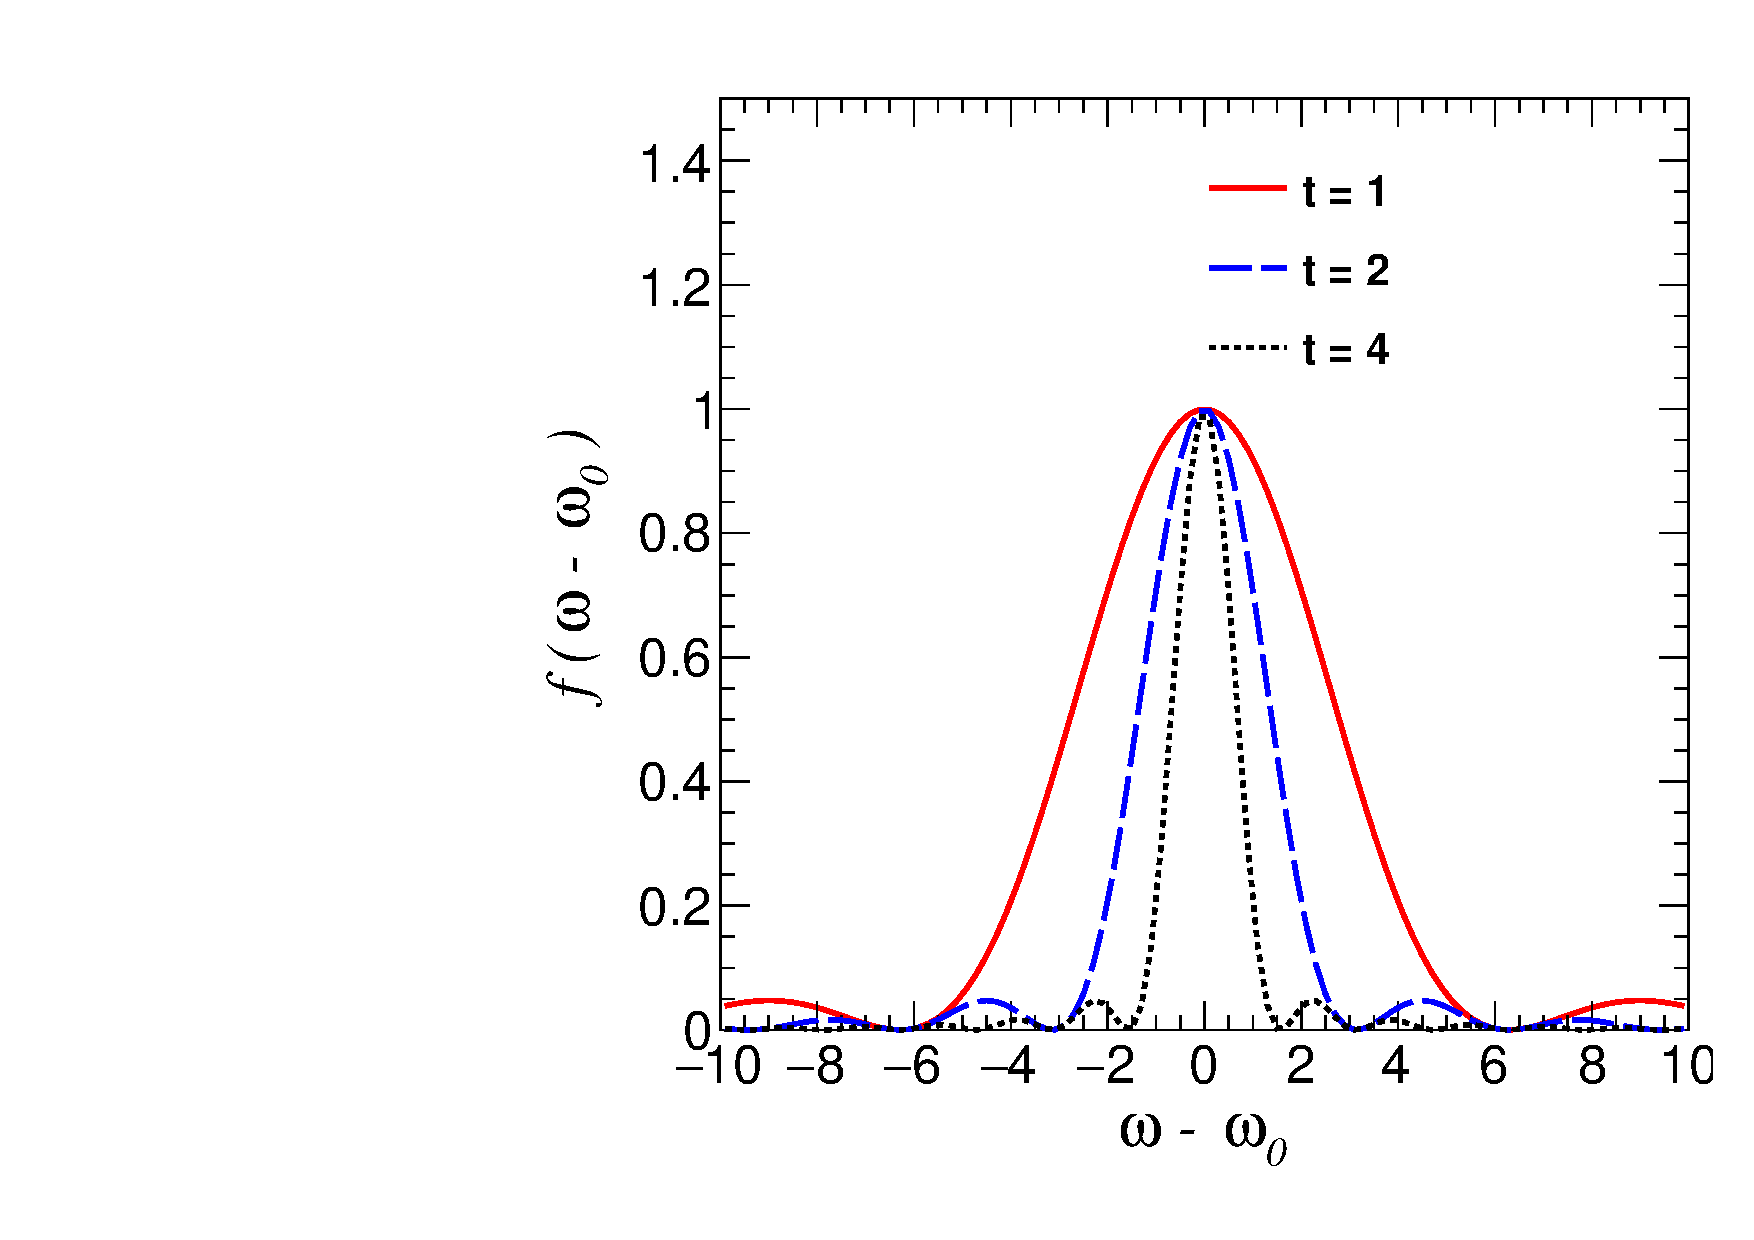
\includegraphics[width=0.5\textwidth]{Figures/fomegaomega0.pdf}\end{center}

So we consider that $f(\omega-\omega_0,t) \xrightarrow{\omega\,\approx\,\omega_0} \frac{2\pi}{t} \delta(\omega-\omega_0)$.
Therefore
\be
p_{i \rightarrow f}(t) = \frac{\lambda^{2}}{\hbar^{2}}\left|A_{f i}\right|^{2} t^2 f(\omega-\omega_0,t)
\label{eq:g58}
\ee
where $p_{i \rightarrow f}(t)$ is related to the transition probability per unit time $\Gamma_{i\to f}$:
\[
\Gamma_{i\to f} = \frac{p_{i \rightarrow f}}{t} = \frac{\lambda^{2}}{\hbar^{2}}\left|A_{f i}\right|^{2} t \times f(\omega-\omega_0,t).
\]

%%% 23 OKAY

This result was derived using perturbation theory,
based on the assumption of $\lambda$ ``small'' and
short times $\to$ 
Eq.~\eqref{eq:g58} is valid only when $p_{i \rightarrow f}(t) \ll 1$.

In practice, not always an isolated final state
$\ket{f}$ is accessible; one needs then to sum over
many or all final states:
\be
\Gamma=\sum_{f} \Gamma_{i \rightarrow f} \rightarrow \int d E D(E) \Gamma(E)
\ee
where the ``sum to integral'' step can be done when levels are densely packed.
$D(E)$ is the density of states (see below).

Using the perturbative result of Eq.~\eqref{eq:g58} in this,
one obtains, for the on-resonance situation,
and already substituting $f(\omega-\omega_0,t) = \frac{2\pi}{t} \delta(\omega-\omega_0)$
\[
\begin{aligned}
\Gamma 
&=\int d E D(E) \frac{\lambda^{2}}{\hbar^{2}} \left|A_{f i}\right|^{2} t \times \frac{2\pi}{t}
\delta\left(\omega-E / \hbar+E_{i} / \hbar\right)\\
&= \frac{\lambda^{2}}{\hbar^{2}} \left|A_{f i}\right|^{2} 2\pi \hbar \, D(\underbrace{E_i + \hbar \omega}_{E_f})
\end{aligned}
\]
so finally
\be
\Gamma  = \frac{2\pi}{\hbar} \lambda^2 \left|A_{f i}\right|^{2} D(E_f)
\ee
This is Fermi's Golden Rule: transition probability rate is independent of time and proportional to the square of the matrix element of the perturbation -- as promised.

%%% 24 OKAY

\subsubsection{Density of states}

(Here we consider noninteracting particles only.)

System in a box of side $L$, under periodic
boundary conditions (p.b.c).
Consider first \emph{one-dimension}:
\be
-\frac{\hbar^{2}}{2 m} \nabla^{2} \psi=E \psi \therefore\left(\frac{d^{2}}{d x^{2}}+k^{2}\right) \psi=0, k^{2}=\frac{2 m E}{\hbar^{2}}
\ee
$\rightarrow$ $\psi(x)=e^{i k x} \quad \psi(x)=\psi(x+L) \Rightarrow e^{i k L}=1$
%
\be
\cos k L=1 \rightarrow k L=2 n \pi \rightarrow k_{n}=\frac{2 n \pi}{L}, n=0, \pm 1 \pm 2, \ldots
\ee
%
\be
E \rightarrow E(n)=\frac{\hbar^{2}}{2 m}\left(\frac{2 \pi}{L}\right) n^{2}
\ee

There are situations (like in the previous discussion)
where one needs to sum over levels. When levels
are close-packed (or in the continuum), sum is replaced
by an integral $\Rightarrow$ this is achieved by taking $L \to \infty$.
\begin{itemize}
\item note that for two consecutive levels
\be
\Delta n=(n+1)-n=1 \Rightarrow \Delta n=\frac{L}{2 \pi} \Delta k_{n}
\ee
%%% 25 OKAY (SKIPPED STEPS)
\item therefore, one can write
\be
\sum_{n} f\left(k_{n}\right)=\sum_{n} f\left(k_{n}\right) \Delta n=\frac{L}{2 \pi} \sum_{n} \Delta k_{n} f\left(k_{n}\right)
\ee
%
\item for $L \to \infty$, $\Delta k_{n}=\frac{2 \pi}{L} \rightarrow dk$ and
$\sum_{n} \rightarrow \int_{-\infty}^{+\infty} d k$ 
\be
\sum_{n} f\left(k_{n}\right) \rightarrow \int_{-\infty}^{+\infty} \underbrace{d k \frac{L}{2 \pi}}%
_{D(k) dk} 
f(k)
\ee
where we identify the $D(k)$ the density of states.
\end{itemize}

For three-dimensions:
\[
\left(\nabla^{2}+k^{2}\right) \psi(x, y, z)=0 \Rightarrow\left(\frac{\partial^{2}}{\partial x^{2}}+\frac{\partial^{2}}{\partial y^{2}}+\frac{\partial^{2}}{\partial y^{2}}+k^{2}\right) \psi=0
\]

(skipped steps)

%%% 26 OKAY (SKIPPED STEPS)
\setcounter{equation}{67}
\be
\psi(\vec{r}\,) = e^{i(k_x x + k_y y + k_z z)} = e^{i \vec{k} \cdot \vec{r}}
\ee
Imposing the p.b.c:
\[
(k_x)_{n_x} = \frac{2 \pi}{L} n_{x}, n_{x}=0, \pm 1, \ldots
\]
and same for $(k_y)_{n_y}$ and $(k_z)_{n_z}$.
The energy, $E=\frac{\hbar^{2} k^{2}}{2 m}$, is then given by
\be
E \rightarrow E\left(n_{x}, n_{y}, n_{z}\right)=\frac{\hbar^{2}}{2 m}\left(\frac{2 \pi}{L}\right)^{2}\left(n_{x}^{2}+n_{y}^{2}+n_{z}^{2}\right)
\ee
%%% 27 OKAY
Sum over levels:
\be
\sum_{n_{x} n_{y} n_{z}} f\left(\left(k_{x}\right)_{n_{x}},\left(k_{y}\right)_{n_{y}},\left(k_{z}\right)_{n_{z}}\right)
\xrightarrow{L \to \infty}
\int d k_{x} d k_{y} d k_{z}\left(\frac{L}{2 \pi}\right)^{3} f\left(k_{x}, k_{y}, k_{z}\right)
\ee
and using that $L^3 = V$
\be
\begin{gathered}
\int \underbrace{d^{3} k\left(\frac{L}{2 \pi}\right)^{3}}%
_{D(\vec{k}) d^3k} f(\vec{k})=\int d^{3} k \frac{V}{(2 \pi)^{3}} f(\vec{k})\\
D(\vec{k}) = \frac{V}{8\pi^3}
\end{gathered}
\ee

\emph{Momentum} density of states:
\[
\vec{p} = \hbar \vec{k} \therefore 
\int d^{3} k \frac{V}{(2 \pi)^{3}} f(\vec{k}) = 
\int d^{3} p \underbrace{\frac{1}{\hbar^3}\frac{V}{(2 \pi)^{3}}}_{D(\vec{p}\,)} f(\vec{p}\,)
\]
therefore
\be
D(\vec{p}\,) = \frac{V}{(2 \pi \hbar)^{3}}=\frac{V}{h^{3}}
\label{eq:g72}
\ee

\emph{Energy} density of states: useful when $f(\vec{p}\,) = f(p)$
\[
\int d^{3} p \frac{V}{(2 \pi \hbar)^{3}} f(p)=\int d p \underbrace{4 \pi p^{2} \frac{V}{(2 \pi \hbar)^{3}}}%
_{D(p)} f(p)
\]
therefore
\be
D(p)=\frac{4 \pi V}{8 \pi^{3} \hbar^{3}} p^{2}=\frac{V}{2 \pi^{2} \hbar^{3}} p^{2}
\ee
%%% 28 OKAY
Using the fact that 
\[
E=\frac{\hbar^{2}}{2 m} k^{2}=\frac{p^{2}}{2 m} \Rightarrow
d E=\frac{p}{m} d p = \frac{\sqrt{2 m E}}{m} d p
\]
we have
\be
\int d p \frac{V}{2 \pi^{2} \hbar^{3}} p^{2} f\left(p^{2}\right)=\int d E 
\underbrace{\frac{d p}{d E} \frac{V}{2 \pi^{2} \hbar^{3}}}_{D(E)} p^{2} f(E)
\ee
with
\[
D(E)=\frac{V}{2 \pi^{2} \hbar^{3}} p^{2} \frac{d p}{d E}=\frac{V}{2 \pi^{2} \hbar^{3}} p^{\cancel{2}} \frac{m}{\cancel{p}}
\]
but
\[
\frac{V}{2 \pi^{2} \hbar^{3}} m p=\frac{V m}{2 \pi^{2} \hbar^{3}}(2 m E)^{1 / 2}
\]
therefore
\be
D(E)=\frac{V m}{2 \pi^{2} \hbar^{3}}(2 m E)^{1 / 2}
\ee
where $D(E)$ is the number of energy levels between $E$ and $E+dE$.

Note that 
\be
V = \int_V d^3r \to d^3r d^3p
\ee
which can be put back in Eq.~\eqref{eq:g72}. So the
number of levels in phase space $(\vec{r},\vec{p})$:
\be
d N=\frac{d^{3} r d^{3} p}{(2 \pi \hbar)^{3}}=\frac{d^{3} r d^{3} p}{h^{3}}
\ee
where $h^3$ is the volume of an elementary cell in phase space.
%%% 29
$\frac{1}{h^3}$: one level per cell
$\Rightarrow$
particle localized within $\Delta x \rightarrow$ momentum $\frac{h}{\Delta x}$,
a quantum particle must have a
volume in phase space as large as $(\Delta x)^{3}(\Delta p)^{3} \sim h^{3}$.

\end{document}
















